% article example for classicthesis.sty
\documentclass[10pt,a4paper]{article} % KOMA-Script article scrartcl
\usepackage{import}
\usepackage{xifthen}
\usepackage{pdfpages}
\usepackage{transparent}
\newcommand{\incfig}[1]{%
    \def\svgwidth{\columnwidth}
    \import{./figures/}{#1.pdf_tex}
}
\usepackage{lipsum}     %lorem ipsum text
\usepackage{titlesec}   %Section settings
\usepackage{titling}    %Title settings
\usepackage[margin=10em]{geometry}  %Adjusting margins
\usepackage{setspace}
\usepackage{listings}
\usepackage{amsmath}    %Display equations options
\usepackage{amssymb}    %More symbols
\usepackage{xcolor}     %Color settings
\usepackage{pagecolor}
\usepackage{mdframed}
\usepackage[spanish]{babel}
\usepackage[utf8]{inputenc}
\usepackage{longtable}
\usepackage{multicol}
\usepackage{graphicx}
\graphicspath{ {./Images/} }
\setlength{\columnsep}{1cm}

% ====| color de la pagina y del fondo |==== %
\pagecolor{black}
\color{white}



\begin{document}
    %========================{TITLE}====================%
    \title{{  Notas tema introduccion AED  }}
    \author{{Rodrigo Castillo}}
    \date{\today}

    \maketitle


     % ====| Loguito |==== %
    
\includegraphics[width=0.1\linewidth]{negro_cara.png}
    %=======================NOTES GOES HERE===================%
    \section{introduccion}
        \begin{itemize}
            \item {la mayoria de problemas involucran varias medidas de
                multiples variables}
            \item {extenderemos algunos metodos bla bla bla}
            \item {muchos problemas de basan den la distribucion normal
                multivariable}
            \item {sirve mucho}
        \end{itemize}

    \section{Organización y nomenclatura}

        utilizaremos la notacion $ x_{ij}  $  como medida de la $ k-esima  $
        variable del $ j-esimo  $ dato u observacion.
        \\ 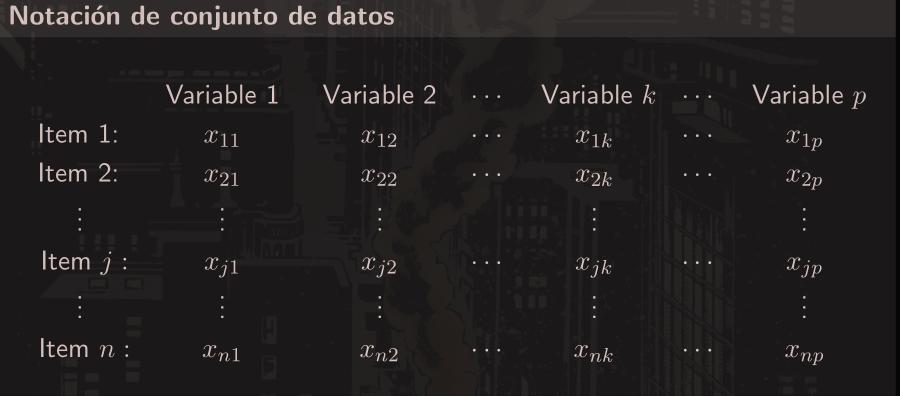
\includegraphics[width=0.5\linewidth]{imagen1.png}

        la notacion de la matriz es :
        \\
        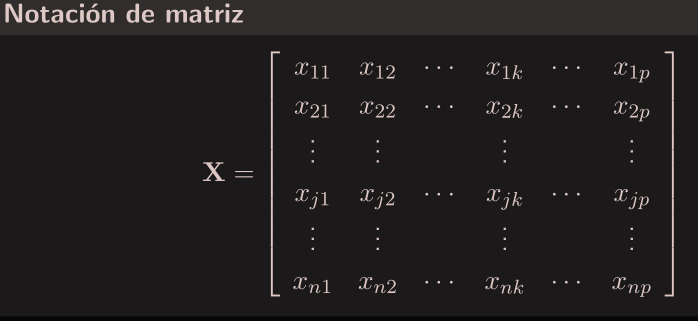
\includegraphics[width= 0.5\linewidth]{matriz.png}

    \section{Estadistica descriptiva}
        \begin{itemize}
            \item {generalmente los conjuntos de datos son grandes}
            \item {toca crear medidas que resuman los datos}
            \item { usualmente se usan medidas que miden \color{red} la
                variacion , la ubicacion y la asociacion lineal \color{white}    }
        \end{itemize}

        Media Muestral:
        \\
        \begin{equation}
            \color{blue} \hat{x_k} = \frac{1}{n}\sum_{j=1}^{n} x_{jk} ,
            k=1,2,3,4,...,p \color{white}
        \end{equation}
        Varianza Muestal:
        \\
        \begin{equation}
            \color{blue} s_k ^{2}  = \frac{1}{n} \sum_{j=1}^{n}(x_{jk} -
            \hat{x_k} )^{2}  ,
            k=1,2,3,4 ... , p \color{white}
        \end{equation}

        otros datos...
        \begin{itemize}
            \item {calcular resumen de los datos}
            \item {promedio de los cuadrados de las distancias de todos los
                numeros con respecto a la media}
        \end{itemize}

        La varianza se puede considerar como la diagonal de una matriz...
        \\
        \begin{equation}
            \color{blue} s_k ^{2}  = s_{kk} = \frac{1}{n} \sum_{j=1}^{n}(x_{jk}
            - \hat{x_k} ) ^{2}   \color{white}  , k = 1,2,3,4,5 , ... ,  p
        \end{equation}
        la raiz cuadrada de la varianza muestral $ \sqrt{s_{kk}}   $ es la
        desviacion estándar

        \begin{itemize}
            \item {la covarianza muestral}
        \end{itemize}
        \begin{equation}
            \color{blue} s_{12} = \frac{1}{n}\sum_{j=1}^{n}(x_{j1} - \hat{x_1}
            )(x_{j2} -
            \hat{x_2} ) \color{white}
        \end{equation}
        y de esto se tiene que
        \begin{itemize}
            \item {es simetrica si $ i = k  $ }
        \end{itemize}

        coeficiente de correlacion muestral :
        \begin{equation}
            \color{blue}  r_{ik} = \frac{s_{ik}}{\sqrt{S_{ii}}\times
            \sqrt{S_{kk}}  } \color{white}
        \end{equation}


        media muestral :
        \begin{equation}
            \color{blue} \hat{X} =  \begin{pmatrix}
                \hat{x_1}
                \\ \hat{x_2}
                \\ .
                \\ .
                \\ .
                \\ \hat{x_p}
            \end{pmatrix}
             \color{white}
        \end{equation}

        covarianzas muestrales :
        \begin{equation}
            \color{blue} S_n = \begin{pmatrix}
                s_{11}  & s_{12} & ... & s_{1p}
                \\ s_{21} & s_{22} & ... & s_{2p}
                \\ . & . & . & .
                \\ . & . & . & .
                \\ . & . & . & .
                \\ s_{p1} ... & ... &  ... &s_{pp}
            \end{pmatrix}
             \color{white}
        \end{equation}
        \color{red} para las Correlaciones muestrales es lo mismo pero con $
        r_{12} , r_{xy}  $  \color{white}

        ejemplo ...
        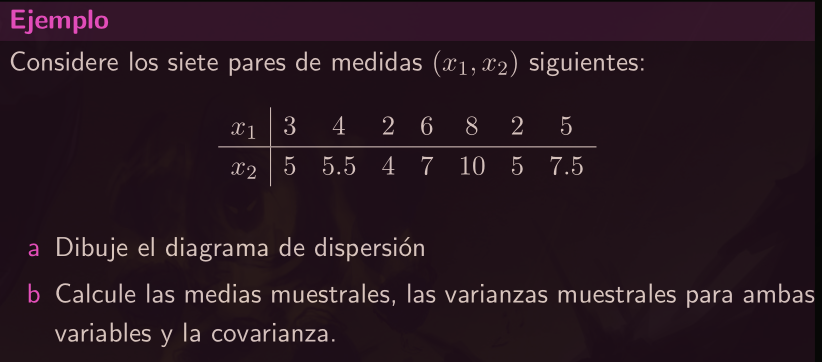
\includegraphics[width=0.8\linewidth]{ejemplo.png}

    \section{Visualizaciones}
        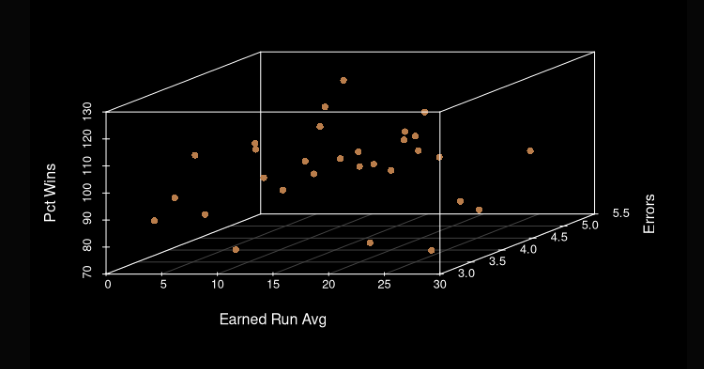
\includegraphics[width=0.5\linewidth]{visu.png}
    \section{Ejercicios}





















    %=======================NOTES ENDS HERE===================%

    % bib stuff
    \nocite{*}
    \addtocontents{toc}{{}}
    \addcontentsline{toc}{section}{\refname}
    \bibliographystyle{plain}
    \bibliography{../Bibliography}
\end{document}
